\section{Auswertung}
\label{sec:Auswertung}




\subsection{Abschwächung des ersten Würfels}
Die gemessenen Zählraten $N$ des ersten Würfels sind in Tabelle 1 dargestellt.

\begin{table}[H]
  \centering
  \caption{Zählrate in Abhängigkeit der Projektion bei einer Messdauer von $\SI{20}{\second}$ }
  \label{tab:Parameter}
  \begin{tabular}{c c c}
    \toprule
    Projektion & $N$ & Fehler   \\
    \midrule
        $I_1$    & 16161 & 152    \\
        $I_2$    & 16165 & 151    \\
        $I_3$    & 16218 & 151    \\
        $I_4$    & 15596 & 151    \\
        $I_5$    & 15662 & 151    \\
        $I_6$    & 15899 & 152    \\
        $I_7$    & 15997 & 153    \\
        $I_8$    & 16187 & 152    \\
        $I_9$    & 16213 & 153    \\
        $I_{10}$ & 15509 & 151   \\
        $I_{11}$ & 15725 & 151    \\
        $I_{12}$ & 15605 & 152    \\
    \bottomrule
  \end{tabular}
\end{table}

Dies sind für weitere Berechnungen die Ausgangszählraten $I_{0,\mathrm{i}}$.




\subsection{Abschwächungskoeffizienten des vierten Würfels}
Die Abschwächungskoeffizienten der einzelenen Materialien werden mit Gleichung (3) bestimmt. Die Dicke
der Elementarwürfel beträgt dabei $d=\SI{1}{\centi\meter}$. In Tabelle (?) werden die gemessenen Zählraten und
die daraus berechneten Abschwächungskoeffizienten dargestellt.

\begin{table}[H]
  \centering
  \caption{Zählrate in Abhängigkeit der Projektion bei einer Messdauer von $\SI{300}{\second}$ und und Abschwächungskoeffizienten }
  \label{tab:Parameter}
  \begin{tabular}{c c c | c c}
    \toprule
    Projektion & $N$ & Fehler & $\mu$ & Fehler   \\
    \midrule
        $I_1$    & 16161 & 152 & &    \\
        $I_2$    & 16165 & 151 & &    \\
        $I_3$    & 16218 & 151 & &    \\
        $I_4$    & 15596 & 151 & &    \\
        $I_5$    & 15662 & 151 & &    \\
        $I_6$    & 15899 & 152 & &    \\
        $I_7$    & 15997 & 153 & &    \\
        $I_8$    & 16187 & 152 & &    \\
        $I_9$    & 16213 & 153 & &    \\
        $I_{10}$ & 15509 & 151 & &   \\
        $I_{11}$ & 15725 & 151 & &    \\
        $I_{12}$ & 15605 & 152 & &    \\
    \bottomrule
  \end{tabular}
\end{table}


\begin{figure}
  \centering
  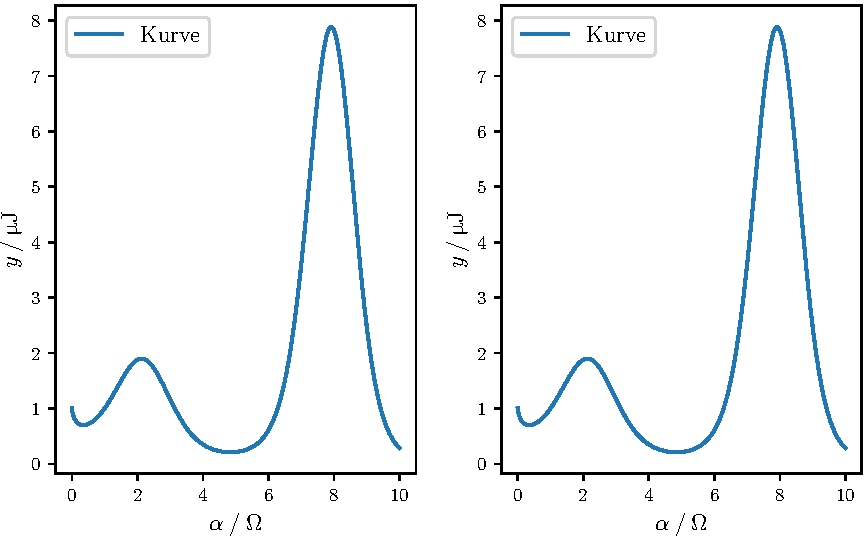
\includegraphics{plot.pdf}
  \caption{Plot.}
  \label{fig:plot}
\end{figure}
